\textbf{Q4. MDPs: Mini-Grids}  \\

The following problems take place in various scenarios of the gridworld MDP.
In all cases, $A$ is the start state and double-rectangle states are exit states.
From an exit state, the only action available is \emph{Exit}, which results in the listed reward and ends the game (by moving into a terminal state $X$, not shown).

From non-exit states, the agent can choose either \emph{Left} or \emph{Right} actions, which move the agent in the corresponding direction.
There are no living rewards; the only non-zero rewards come from exiting the grid.

Throughout this problem, assume that value iteration begins with initial values $V_0(s) = 0$ for all states $s$.

First, consider the following mini-grid.
For now, the discount is $\gamma = 1$ and legal movement actions will always succeed (and so the state transition function is deterministic).

\begin{center}
\centering
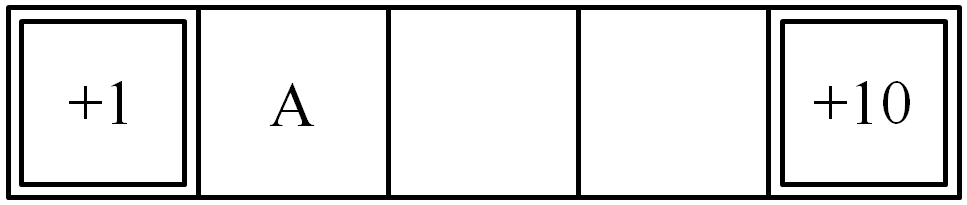
\includegraphics[width=0.4\textwidth]{figures/minigrid-discount.png}
\end{center}

\begin{enumerate}
\item What is the optimal value $V^*(A)$? 
\vfill
\item When running value iteration, remember that we start with $V_0(s)=0$ for all $s$.
What is the first iteration $k$ for which $V_k(A)$ will be non-zero?
\vfill

\item What will $V_k(A)$ be when it is first non-zero?
\vfill

\item After how many iterations $k$ will we have $V_k(A) = V^*(A)$?  If they will never become equal, write \emph{never}.
\vfill

\newpage
Now the situation is as before, but the discount $\gamma$ is less than $1$.
\item If $\gamma = 0.5$, what is the optimal value $V^*(A)$?
\vfill

\item For what range of values $\gamma$ of the discount will it be optimal to go \emph{Right} from $A$?
\vfill

\end{enumerate}
